\section{Algorithme de Grover}
\label{part1}

L’algorithme de Grover est un algorithme de recherche quantique permettant de rechercher un élément parmi $N$ non classés en $\mathcal{O}(\sqrt{N})$.
Dans les mêmes conditions, un algorithme de recherche classique même probabiliste ne peut faire mieux qu'une recherche en $\mathcal{O}(N)$. \cite{grover1996fast}. 
 
\subsection{Description}

Plus formellement, soit $N \in \mathbb{N}, \ \omega \in [\![0, N-1]\!]$ et $f = \mathbbm{1}_{\{ \omega \}}$ la fonction indicatrice de la \textit{solution} $\omega$.
L'algorithme de Grover consiste à trouver $\omega$ dans l'ensemble $[\![0, N-1]\!]$ en utilisant seulement un nombre d'appel à la fonction $f$ proportionnel à $\sqrt{N}$. 
\\
Pour ce faire, nous représentons les éléments de $[\![0, N-1]\!]$ dans $\mathcal{H} = (\mathbb{C}^2)^{\otimes n}$, un espace de Hilbert de dimension $2^n$, qui peut être implémenté par un registre quantique utilisant $n=\lceil{log_{2} N} \rceil$ qubits.\footnote{Notons que si $N$ n'est pas une puissance de 2, certaines dimensions (et par conséquent, certains qubits) de $\mathcal{H}$ ne sont pas utilisées. }
\\
Plus précisément, il s'agit de l'isomorphisme:
\begin{align*}
	\Phi : [\![0, N-1]\!] &\longrightarrow \mathcal{H} \\
	x &\longmapsto | x \rangle = | B(x, n)\rangle
\end{align*}
Où $B(x, n)$ est la représentation en base 2 de $x$ codée sur $n$ bits.\footnotemark
\footnotetext{Pour $x=3$ et $N=7$ par example, on a $\Phi(2) = |010\rangle = |0\rangle \otimes |1\rangle \otimes |0\rangle \in (\mathbb{C}^2)^{\otimes 3}$ }
\\
Notons que les états $| x \rangle$ forment une base orthonormée de $\mathcal{H}$, en effet il s'agit des composantes de la base canonique de $(\mathbb{C}^2)^{\otimes n}$.
Nous définissons par la suite l'opérateur unitaire $U_{\omega}$ (appelé oracle) de sorte que $U_{\omega}|x\rangle = (-1)^{f(x)}|x\rangle$. 
\\
L'algorithme retourne ainsi $\omega$ avec une probabilité supérieure à 1/2 en utilisant $\mathcal{O}(\sqrt{N})$ appels à $U_{\omega}$. De plus, cette probabilité converge vers 1 en augmentant le nombre d'exécutions.

\subsection{Algorithme}
Soit $r\in \mathbb{N}$ l'entier le plus proche de $\frac{\pi}{4} \sqrt{N}$.
\begin{itemize}
	\item[1] Initialiser le système à la superposition uniforme de tous les états:
	\begin{align}
	|\psi \rangle = |\psi_{(0)}\rangle = \frac{1}{\sqrt{N}} \sum_{k=0}^{N-1} |k\rangle
    \label{init}
	\end{align}
	\item[2] Appliquer l'itération de Grover $r$ fois:
	\item[] Pour $i \in [\![0, r-1]\!]$,
	\begin{itemize}
   	 
    	\item[2.1] Appliquer à $|\psi_{(i)}\rangle$ l'oracle $U_{\omega}$, donné aussi par la formule:
    	\begin{align}
    	U_{\omega} = Id -  2|\omega \rangle \langle \omega |
    	\label{Uomega}
    	\end{align}
    	\item[2.2] Appliquer à $|\psi_{(i)}\rangle$ l'opérateur de diffusion de Grover $U_{\psi}$ :
    	\begin{align}
    	U_{\psi} = 2|\psi\rangle \langle \psi | - Id
        \label{Upsi}
    	\end{align}
	\end{itemize}
	\item[] On se retrouve donc avec $|\psi_{(i+1)}\rangle = U_{\psi}U_{\omega} |\psi_{(i)} \rangle$. 
	\item[3] Mesurer l'état résultant $|\psi_{(r)} \rangle$.
\end{itemize}

\noindent Moralement, l'algorithme consiste à effectuer une série de rotations sur l'état $|\psi \rangle $ afin qu'il se rapproche au maximum de l'état $|\omega \rangle $ dans l'espace vectoriel $\mathcal{H}$, comme illustré par la figure \ref{fig:grover}. 
Cela permet donc, lors la mesure de l'état résultant, l'obtention de l'état recherché avec haute probabilité. 
On observe qu'à chaque itération, l'algorithme amplifie l'amplitude\footnotemark \, du vecteur $|\omega\rangle$ superposé dans le vecteur $|\psi\rangle$. Cette amplification donne nom à la technique généralisante de l'algorithme de Grover et nous fournit également l'illustration \ref{fig2:subfigures} présentée en annexe.

\footnotetext{Pour un vecteur d'état $|\psi\rangle$ se décomposant comme une combinaison linéaire (superposition) de vecteurs: $|\psi\rangle = \sum_i \alpha_i |\psi_i\rangle$, on appelle amplitude les nombres complexes $\alpha_i$. La probabilité d'obtenir un vecteur $|\psi_i\rangle$ lors d'une mesure est donnée par $|\alpha_i|^2$, ce qui nous donne $\sum_i |\alpha_i|^2 = 1$. }


\subsection{Preuve de validité}

L'algorithme débute avec $|\psi \rangle \in F = \mathrm{Vect}(|\psi \rangle , |\omega \rangle ))$. 
\\
Par le procédé d'orthonormalisation de Gram-Schmidt, nous avons $(|\psi' \rangle, | \omega \rangle)$ une base orthonormale de $F$ avec 
\[|\psi'\rangle = \frac{1}{\sqrt{N-1}}\sum_{x \neq \omega} |x \rangle\]
la projection orthogonale de $|\psi \rangle$ sur $\mathrm{Vect}(|\omega \rangle ))^{\perp}$, normalisée. 
\\
L'opérateur $U_{\omega}$ est une symétrie orthogonale par rapport à l'hyperplan $\mathrm{Vect}(|\omega \rangle)^{\perp}$, ce qui explique la formule donnée par \eqref{Uomega}. C'est donc en particulier une symétrie par rapport à $|\psi'\rangle$ pour les éléments de $F$.
L'opérateur $U_{\psi}$ donnée par \eqref{Upsi} est une symétrie orthogonale par rapport à $|\psi\rangle$.
On remarque aussi que $F$ est stable par $U_{\omega}$ et $U_{\psi}$, ainsi les états $|\psi_{(i)} \rangle$ restent dans le sous espace vectoriel $F$ durant la totalité de l'exécution de l'algorithme.
\\
À chaque itération, l'opérateur $Q=U_{\psi} U_{\omega}$ réalise une rotation de $2\theta$ avec:
\[\theta = \mathrm{arcsin}(\frac{1}{\sqrt{N}})\]
Donc avec assez de rotations, nous pouvons orienter l'état de départ vers $|\omega \rangle$.
Cependant, il est cruciale d'arrêter l'algorithme quand le vecteur d'état se rapproche de $|\omega \rangle$, car en ayant dépassé l'état ciblé, les rotations postérieurs éloigneront $|\psi_{(i)} \rangle$ de $|\omega \rangle$.
La probabilité exacte de la mesure est donnée par:
\[\mathrm{sin}^2 \left( \left( 2r + 1 \right) \theta \right) \]
Nous expliquerons cette valeur par la suite. 
\begin{figure}
\centering
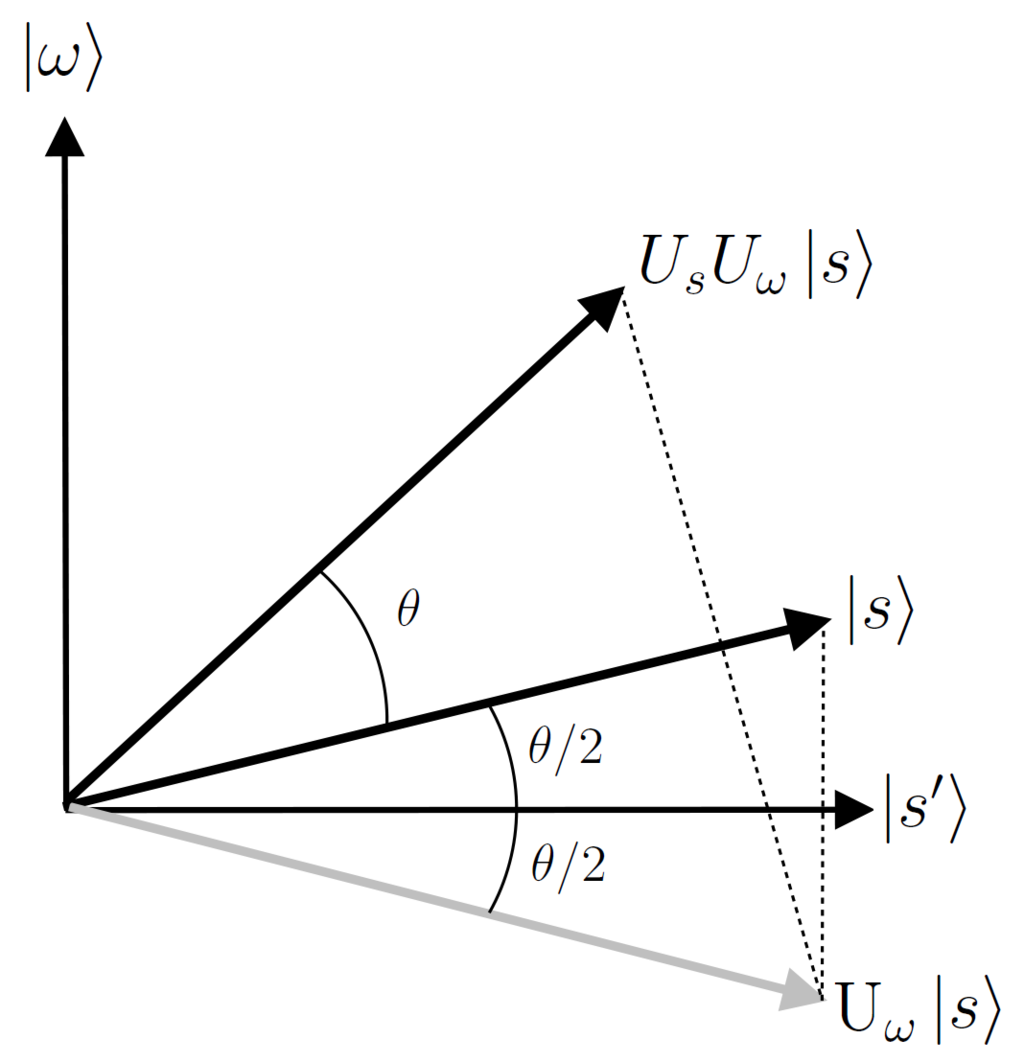
\includegraphics[scale=0.5]{Grovers_algorithm_geometry}
\caption{Interprétation géométrique  de l'algorithme de Grover}
\label{fig:grover}
\end{figure}



